\documentclass{standalone}
\usepackage{tikz}
\tikzset{block/.style = {draw, fill=white, very thick, rectangle, minimum height=1cm, minimum width=2cm}}
\begin{document}
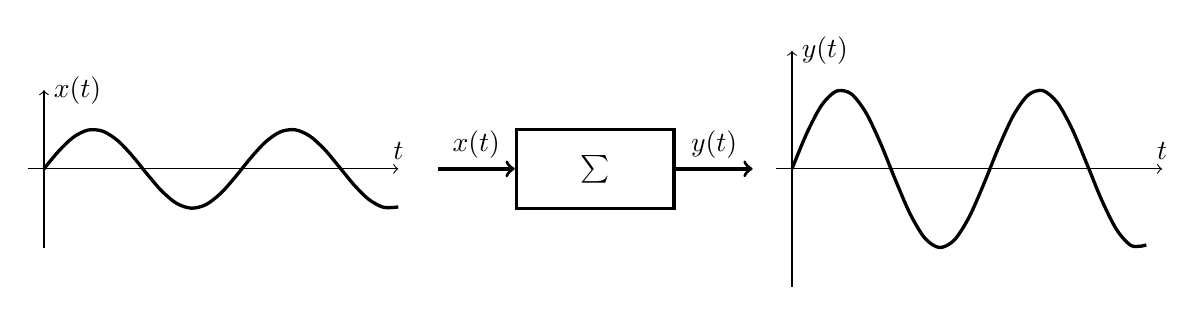
\begin{tikzpicture}[scale=2]
    \node[block](s)at(0,0){$\sum$};
    \draw[->](-3.6,0)--(-1.25,0)node[above]{$t$};
    \draw[->](-3.5,-0.5)--(-3.5,0.5)node[right]{$x(t)$};
    \draw[-,very thick]plot[smooth, domain=-3.5:-1.25](\x,{0.25*sin(5*(\x+3.5) r)});
    \draw[->,very thick](-1,0)--(s.180)node[midway, above]{$x(t)$};
    \draw[-,very thick]plot[smooth, domain=1.25:3.5](\x,{0.5*sin(5*(\x-1.25) r)});
    \draw[->](1.15,0)--(3.6,0)node[above]{$t$};
    \draw[->](1.25,-0.75)--(1.25,0.75)node[right]{$y(t)$};
    \draw[->,very thick](s.0)--(1,0)node[midway, above]{$y(t)$};
\end{tikzpicture}
\end{document}